
%(BEGIN_QUESTION)
% Copyright 2006, Tony R. Kuphaldt, released under the Creative Commons Attribution License (v 1.0)
% This means you may do almost anything with this work of mine, so long as you give me proper credit

Some bourdon tube gauges are equipped with a very small spiral spring attached to the pointer shaft:

$$\includegraphics[width=15.5cm]{i00175x01.eps}$$

Now, this spring is much too weak to have any detectable effect on the span of the gauge.  In other words, it does not measurably resist the bending action of the bourdon tube, as a ``range spring'' would in another design of instrument.

Given its weakness, what possible purpose does this spring serve in the gauge mechanism?

\vskip 10pt

\underbar{file i00175}
%(END_QUESTION)





%(BEGIN_ANSWER)

It is an ``anti-backlash'' spring, supplying enough torque to rid the sector/pinion gear set of any ``slack'' or ``play,'' so that the pointer always responds to the slightest change in bourdon tube position.

%(END_ANSWER)





%(BEGIN_NOTES)

Another tactic for eliminating backlash in geared instruments is to use a set of side-by-side gears placed under tension by a coiled spring, both gears meshing with a common (driving) gear.  With two gears meshing against the one, each of the two gears with an opposing torque, there will be no ``looseness'' in the gear train to create deadband or hysteresis in the pointer motion.

If absolutely backlash-free motion transfer is desired, gears may be replaced by wheels coupled by spring-steel straps in a precision mechanism.  Such drive linkages are frequently used in computer hard-drive head positioning mechanisms.  The idea of using a flexible metal ribbon as a backlash-free joint is not unique to rotary motion: when used as small-angle pivots, such straps are called {\it flexures}.

%INDEX% Measurement, pressure: bourdon tube (anti-backlash spring)

%(END_NOTES)


